\newpage
\section{Degustation}
\subsection{Planung}
\subsubsection{Ziel der Degustion}
\begin{itemize}
    \item Erkennen die Befragten den Unterschied zwischen alkoholfreiem und alkoholhaltigem Bier?
    \item Können wir als Anfänger ein vergleichbares Bier herstellen?
    \item Wie wird unser Bier bewertet?
\end{itemize}
\textbf{Auswertungsblatt}\\
Die Auswertungs Blatt ist in den Beilagen sichtbar.
\subsubsection{Durchführung}
Wir verwenden Plastikbecher und markieren diese mit folgendem Farbschema:
\begin{itemize}
    \item Blau: 	Selbstgebrautes Weizenbier
    \item Rot:		Selbstgebrautes Cherry Ale
    \item Gelb: 	Feldschlösschen Braufrisch \cite{brack}
    \item Grün:		Chouffe Cherry Ale \cite{Manor}
    \item Schwarz:	Appenzeller Weizenbier (Alkoholfrei) \cite{Coop}
\end{itemize}
\paragraph{}
Danach werden die Biersorten in die dafür vorgesehenen Plastikbecher abgefüllt. Es soll somit vermieden werden, dass die Teilnehmer wissen, um welches Bier es sich jeweils handelt.
Wir bitten die Teilnehmer dann jeweils eine Biersorte nach der anderen zu probieren und dabei das Auswertungsblatt, welches weiter unten zu finden ist, auszufüllen. Mit dieser Methode ist es uns möglich herauszufinden, ob die Testpersonen unser Bier mögen oder einen Unterschied von alkoholhaltigem und nicht alkoholhaltigem Bier herausschmecken können. Weiter werden wir bei der Wahl darauf achten, möglichst unterschiedliche Altersgruppen und Alkoholkonsumenten einzuladen, so dass wir gegebenenfalls einen Unterschied zwischen Altersgruppen und den verschieden starken Alkoholkonsumenten herausfinden können.
\\
\textbf{Design:}\\
Aktuell haben wir nur die «nackten» Bierflaschen. Da wir aber bei der Degustation und vor allem auch bei der Präsentation einen ästhetisch ansprechenden Auftritt liefern wollen, haben wir und dazu entschieden Labels für die Flaschen zu erstellen. Diese Aufgabe haben wir mit Photoshop und Etikettenpapier bewältigen. Wir haben mehrere Designs erstellt und uns für die zwei folgenden entschieden:

\begin{figure}[!h]
    \centering
    \begin{minipage}{.5\textwidth}
      \centering
      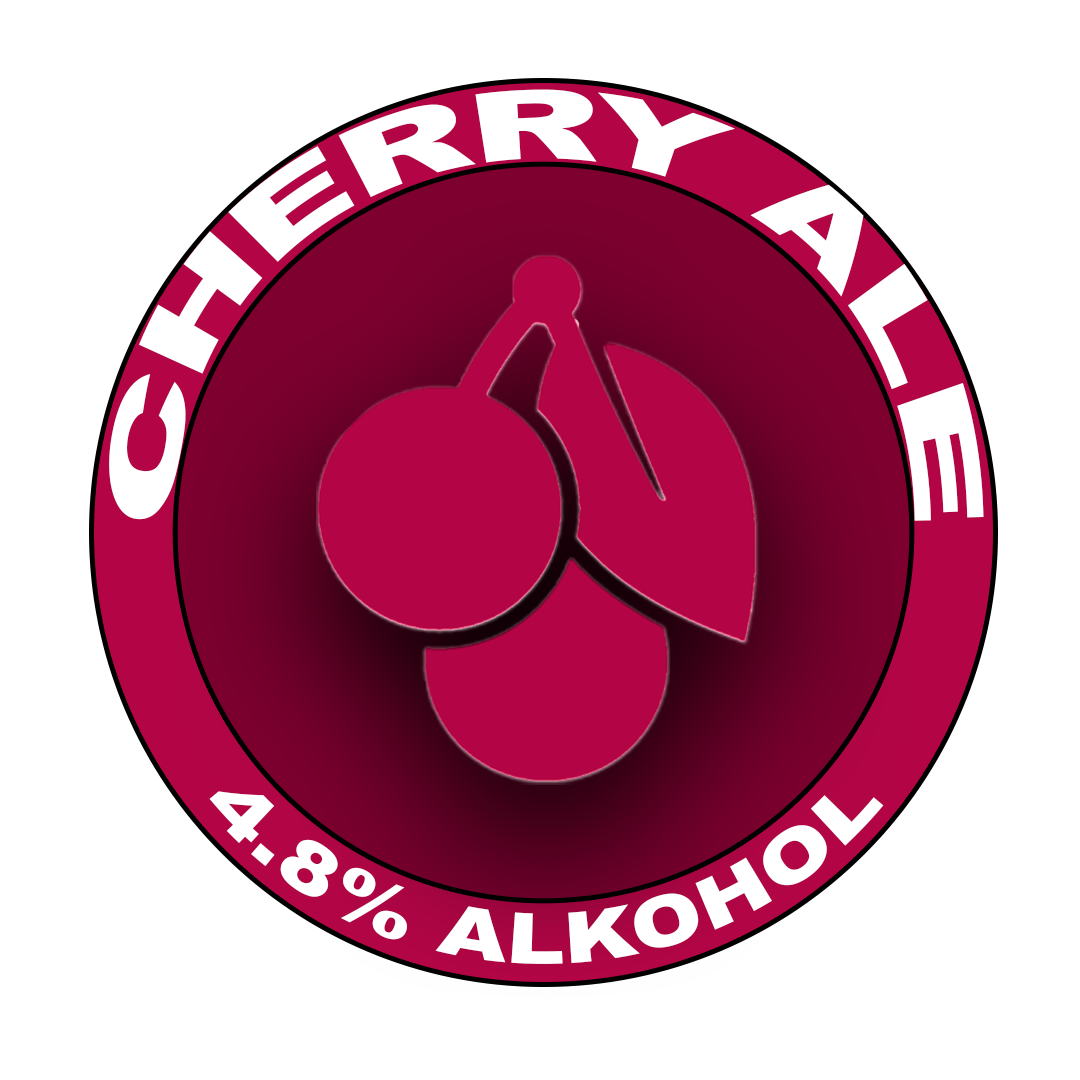
\includegraphics[width=.7\linewidth]{Cherry.png}
      \captionof{figure}{Cherry Ale Design}
      \label{fig:test1}
    \end{minipage}%
    \begin{minipage}{.5\textwidth}
      \centering
      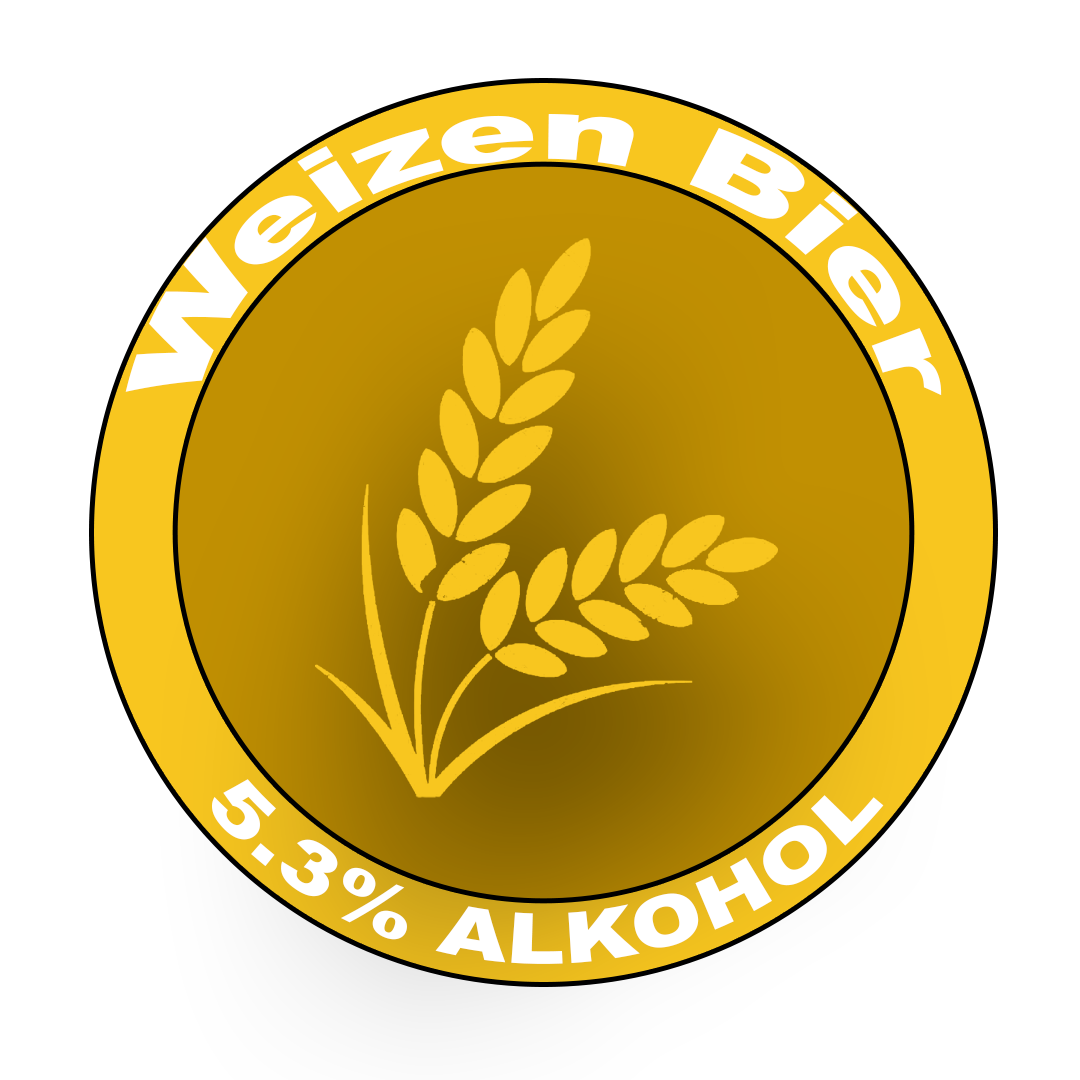
\includegraphics[width=.7\linewidth]{Figures/Wheat.png}
      \captionof{figure}{Wheat Design}
      \label{fig:test2}
    \end{minipage}
\end{figure}

\textbf{Allgemein:}
Es war uns wichtig, dass das Design simpel und ansprechend aussieht. Dazu waren wir limitiert, da unser Etikettenpapier uns nicht viel Platz bat. Da wir das Bier nicht kommerziell nutzen, mussten wir auch keine Angaben über die Inhaltsstoffe andrucken, was uns natürlich viel Ärger erspart hat. Der Äussere Ring dient als Platzhalter für den Titel und den Alkoholgehalt. In der Mitte haben wir einen dunkleren Hintergrund und das Logo, welches mit einem leichten Schlagschatten heraussticht.
\\
\textbf{Cherry Ale:}
Die Kirsche vom Cherry Ale Logo wurde von dem Unternehmen «MX CHERRY» \cite{Cherry}  inspiriert. Farblich haben wir uns für ein dunkles Weinrot entschieden, da wir fanden, dass das zu Kirschen passen würde. Der kapitalisierte und verzerrte Titel sorgt für Aufmerksamkeit und das Logo sticht von der Mitte hervor.
\\
\textbf{Weizen Bier:}
Beim Weizenbier wollten wir natürlich auch in dem gleichen Stil bleiben, jedoch sollte jedermann einen klaren Unterschied zwischen den Biersorten erkennen. Dies haben wir mehrheitlich durch die Farbe und dem Symbol erzeugt. Hier haben wir die Kapitalisierung des Titels weggelassen, um dem Symbol eine grössere Aufmerksamkeit zu widmen. 
